\chapter{System Design}
In this chapter we will discuss the architecture and design of the \textbf{TechBook} system. In the following sections we will present code snippets and visual diagrams to help portray a basic understanding of the application design. The architecture is modeled on what is known as the MEAN stack and which resembles a three tier architecture. MEAN is a free open-source software stack for building dynamic websites and supports the MVC (Model View Controller) architecture. The contents of this chapter will be begin with a brief overview of the flow of the MEAN stack followed by a more in depth portrayal separated into the Data Tier, Logic Tier and Presentation Tier.

\section{Overview}
The Presentation tier uses Angularjs, being a client side JavaScript language it is the the first one to process the request made by the client. The request is then sent to the Logic-tier which is a Nodejs server side JavaScipt language. Then the request enters the third phase using ExpressJS to make a request to the Data tier.

From that point, the data is retrieved  from the MongoDB and the response is returned to Expressjs. Finally NodeJS takes the data back from ExpressJS and the data is returned to the Presentation tier to display the result.


\begin{figure}[H]
\begin{minipage}{.4\textwidth}  %listing bloc will have 50% of the line width 
\lstset{linewidth = 4cm, breaklines=true} %set your listing lines widths, and set breaklines to true
\begin{itemize}
\item Database \textbf{MongoDB}
\item Server \textbf{Node.js/express}
\item Client \textbf{Angular.js}
\end{itemize}

\end{minipage}
\qquad %space between listing bloc and the figure
\begin{minipage}{0.6\textwidth} %figure will have the remaning 40% of the line width
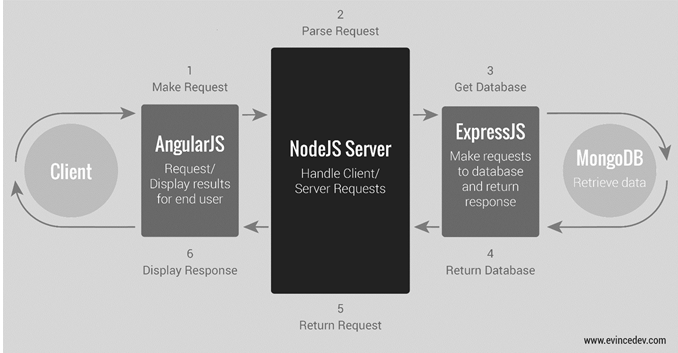
\includegraphics[scale=.4]{img/mvc.png} %the image must be resized or scaled if needed
\caption{MEAN Stack}
\end{minipage}
\end{figure}

% ========================== Databases ========================== 
\section{Data Tier}
For the database adapting the MEAN architecture we used MongoDB.

\subsection{Mongoose}
Harnessing the true power of the Mean stack we used the mongoose object modelling package for Node. Mongoose enabled us to have access to the full suite of MongoDB commands to perform CRUD (Create, Read, Update, Delete) operations. 


To use mongoose we must first connect the logic tier to the data tier. We used the following command in the project directory to add it to our Node project:
\begin{minted}{console}
npm install mongoose --save
\end{minted}

Once the package was installed we have to access it in our project :
\begin{lstlisting}[language=JavaScript]
var mongoose = require('mongoose');
\end{lstlisting}

Finally to connect to our MongoDB:
\begin{lstlisting}[language=JavaScript]
// Connect to the mongodb using settings from the config file
mongoose.connect(config.database, { promiseLibrary: require('bluebird') })
  .then(() =>  console.log('\x1b[32m%s\x1b[0m', 'INFO: Connection to database succesfull'))
  .catch((err) => console.error(err));
\end{lstlisting}

\subsection{Mongoose Schema}
Prior to performing CRUD operations we had to define our  mongooses models. These represent documents which can be saved, read and retrieved from our database. The Mongoose Schema is how we define attributes to these documents. To enhance security and the SRP(Single Responsibility Principle) numerous different models were defined and using keys enabled the ability to map relationships to other models.

\begin{figure}[H]
  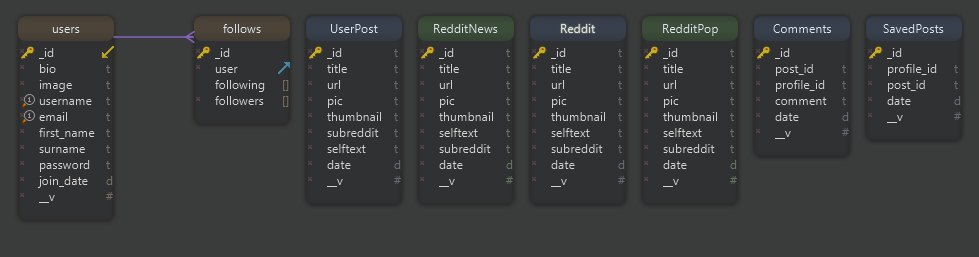
\includegraphics[width=\linewidth]{img/schemas.PNG}
  \caption{MongoDB models}
  \label{fig:schema}
\end{figure}

Figure ~\ref{fig:userscema} below shows how the UserSchema was defined in user.js. The schema was designed to add maximum functionality while also protecting the system from having invalid objects added to the database. There are a few things to note about this particular schema.
\begin{itemize}
\item \textbf{Uniqueness} : The \textit{username} and \textit{email} fields are set to unique. This ensures a user can only have one account per email and that the username will not not cause issues when a search query is performed.
\item \textbf{Required} : The \textit{username}, \textit{firstname},\textit{surname} and \textit{password} fields are required. These represent the bare minimum that must be initialised to have a valid account.
\item \textbf{Default} : The \textit{joindate},\textit{bio} and \textit{image} are set to default. This allows a faster user registration with a default image used, the join date set to the current date and a generic bio that can all be updated using the settings link.
\end{itemize}

\begin{lstlisting}[language=JavaScript,caption={Defining User Schema},captionpos=b,label={fig:userscema}]
// Schema used to 'filter' data to be stored in the 'UserSchema' collection in mongo
var UserSchema = new mongoose.Schema({
  username: {
    type: String,
    unique: true,
    required: true
  },
  email: {
    type: String,
    unique: true,
  },
  first_name: {
    type: String,
    required: true
  },
  surname: {
    type: String,
    required: true
  },
  join_date: {
    type: Date,
    default: Date.now
  },
  bio: {
    type: String,
    default: 'Tell me about yourself'
  },
  image:{
    type: String,
    default: 'profile.jpg'
  },
  password: {
    type: String,
    required: true
  }
});

\end{lstlisting}

\subsection{Password hashing}
To ensure the highest standard of security any confidential user information should never directly be stored in a database. Mongoose allows us to define functions using 'pre(function,functionToExecute)' that executes prior to saving a document. Bcrypt a node-module that simplifies hashing can be used to both encrypt and decrypt sensitive data. Combining the use of these technologies when a user account is created or modified, the password is hashed before saving the document and in turn the hashed value of the password is saved in the database thus protecting the origonal password being exposed in the event of a malicious attack.

\begin{lstlisting}[language=JavaScript,caption={Password Hashing},captionpos=b,label={fig:presave}]
// define pre hook for document
UserSchema.pre('save', function (next) {
  var user = this;
  // if password new or edited
  if (this.isModified('password') || this.isNew) {
    // generate a salt and process data for 10 rounds
    bcrypt.genSalt(10, function (err, salt) {
      if (err) {
        return next(err);
      }
      // generate a hash of password
      bcrypt.hash(user.password, salt, null, function (err, hash) {
        if (err) {
          return next(err);
        }
        user.password = hash;
        next();
      });
    });
  } else {
    return next();
  }
});

\end{lstlisting}
Ensuring the password is hashed is of major importance but equally as crucial is the ability to be able to compare the hashed value with a password entered by a user attempting to log in. To achieve this we were able to attach a comparePassword function to the UserSchema which executes the compare method from the bcrypt module and checks for a match between the password entered and the hashed password stored in the database as shown in Figure ~\ref{fig:passcheck}. 
\begin{lstlisting}[language=JavaScript,caption={Password Comparision},captionpos=b,label={fig:passcheck}]
// compare password for log in
UserSchema.methods.comparePassword = function (passw, cb) {
  bcrypt.compare(passw, this.password, function (err, isMatch) {
    if (err) {
      return cb(err);
    }
    cb(null, isMatch);
  });
};
\end{lstlisting}

\section{Logic Tier}

The Logic tier is where the Web API service acts as the doorway to all business logic and data storage.
Here we perform more complicated computations and sequencing of events allowing us to manipulate data by creating, reading, updating or deleting. Some events are user driven such as editing a profile and some run periodically such as generating posts from the Reddit API. Due to NodeJS's non-blocking IO calls and light-weight implementation, its enables the application to scale handling thousands of concurrent connections. Being written in the NodeJS JavaScript it is perfect for connecting our Data tier to our Presentation tier. The Logic tier also provides authentication to ensure no unauthorised acces is given to the database.

% ========================== Authentication ========================== 
\subsection{Authentication}
With the purpose of security and the recent rise in data leaks making social media the biggest data breach threat \cite{dataleaks} the application was designed to secure data when a user is calling protected API routes.

At a high level the components of the authentication flow are as follows:
\begin{itemize}
    \item The user data is stored in MongoDB, with the passwords hashed prior to saving.
    \item CRUD functions are built in an Express API such as login, register, get profile and update. 
    \item The Angular application calls the API and deals with the responses.
    \item The Express API generates a JSON Web Token upon registration and passes this to the Angular application when a user succesfully logs in.
    \item The Angular application stores the JWT in local storage to maintain the user’s session.
    \item The Angular application checks the validity of the JWT when displaying protected views.
    \item The Angular application passes the JWT back to Express for validation when calling protected API routes.
\end{itemize}
   
% ========================== JSON Web tokens ========================== 

\subsection{JSON Web Tokens}
For the purpose of security we used JSON Web tokens to validate that a legitimate user is logged into the system and prevent unauthorised access. \textit{JSON Web Tokens are an open, industry standard RFC 7519 method for representing claims securely between two parties}\cite{jwt}. A unique JWT token is created in accordance with the offical JWT standard. A users token is signed with the username, password and an expiration date that renders the token invalid after a specified time has passed as seen below. To add to the security the Token is also signed with a secret key defined in the \textit{database.Js} class so that a user cannot simple try to recreate their own version of a token.

\begin{lstlisting}[language=JAVASCRIPTcaption={Creating a JSON Web Token},captionpos=b,label={fig:jwttoken}]
// Method to generate JWT token
UserSchema.methods.generateJWT = function () {
  var today = new Date();
  var exp = new Date(today);
  exp.setDate(today.getDate() + 60);

  return jwt.sign({
    id: this._id,
    username: this.username,
    exp: parseInt(exp.getTime() / 1000),
  }, config.secret);
};
\end{lstlisting}

This token can be used for many types of verification. On the client or presentation tier the JWT is returned from the server after a user has successfully logged in and is stored in local storage. This allows the system to check validity of the user further allowing the restriction/ restriction of components. For more on how the \textit{Json Web Tokens} are used on the presentation tier see Section \ref{loginpage}.

% ========================== Server Logging ========================== 
\subsection{Server Logging}
For development and operation purposes we created a Node module log system on the server. A server logging system boasts many advantages for both the debugging and monitoring the API of the application. By setting up an exportable logger in the \textit{config} folder and importing the logger into the API routes, we can easily debug and monitor information and errors on the server.

The logs required for the system were information logs, error logs and debug logs. The logs are located in \textit{logs} directory on the server and separated into \textit{debug.txt}, \textit{info.txt} and \textit{error.txt}. When a call to log a message is executed  the appropriate file is appended with a time stamp and the message. Figure \ref{fig:serverlogger} displays a shortened version of the logging implementation.

\begin{lstlisting}[language=JAVASCRIPT,caption={Server Logging},captionpos=b,label={fig:serverlogger}]
// Make logger exportable so any file can reference it
var Logger = (exports.Logger = {});

// Creates folder for logs if one doesn't exsist
if (!fs.existsSync('./logs')){
    fs.mkdirSync('./logs');
}

// Create 3 write streams to allow to append info, error and debug logs to different streams.
var errorStream = fs.createWriteStream("./logs/error.txt");

// Append error message to log file along with the current date
Logger.error = function(msg) {
  var message = new Date().toISOString() + " : " + msg + "\n";
  errorStream.write(message);
};
\end{lstlisting}

To use the logger we simply call the error/debug/info function as shown in Figure \ref{fig:serverlog} when an error occurs following a failed registration.

\begin{lstlisting}[language=JAVASCRIPT,caption={Server Log call from API},captionpos=b,label={fig:serverlog}]
// Import logger to handle server logging. 
var logger = require("../config/serverlogger").Logger;

if (!req.body.username || !req.body.password) {
    logger.error("[Register] : user attempted signup with no username or password");
    res.json({
      success: false,
      msg: 'Please enter username and password.'
    });
  }
\end{lstlisting}

The message is then appended to the log file allowing us to easily view the activity on the server. Below is an example of the \textit{error.txt} after an error has been logged.

\begin{lstlisting}[language=JAVASCRIPT,caption={error.txt log file},captionpos=b,label={fig:errorlog}]
2019-04-10T18:30:49.616Z : [Register] : user attempted register with duplicate username
2019-04-10T18:30:49.616Z : [Register] : user attempted register with duplicate email
2019-04-10T18:30:49.616Z : [Login] : user attempted login with incorrect password
2019-04-10T18:30:49.616Z : [Register] : user attempted signup with no username or password
\end{lstlisting}

% ========================== API Calls ========================== 
\subsection{API/HTTP}
How we designed api calls/
insert info from swagger

% ========================== UI ========================== 
\section{Application Tier}
The presentation tier is based on the Angular front-end web framework. In contrast to traditional multiple page web applications the Client is presented as a single page application in which components are injected into. In this section we will look at the Angular app structure, the services which allow us to interact with our node js server and the finished view of the pages.

\subsection{Angular folder structure}

\subsection{Angular Services}
The Angular services allow our application to interact and access data from our database via the node server. Thus keeping data retrieval separate to page functions. In the services we provide the logic to process HTTP requests to the API to perform CRUD operations on the data served by the Node.js/ExpressJS server. 

\subsection{Page views}
In this section we will look at some screen shots of the web application from the view of a PC web browser and on a Samsung Galaxy S6 mobile device. For each page a brief summary of the functionality of the page will be provided along with any input validation that was used. 
How we designed the ui
few screenshots off finished site


\subsubsection{Navigation Pane}
The header component is injected into the main index.js view. This allows us to render the navigation pane at all times while the main content view is adapted to the selected page view. The header component contains a header logo displaying the image that was designed for the application and a navigation bar with numerous features. When designing the navbar we decided it must meet the following conditions: appealing, easy to use and fully functional, all whilst being fully responsive to changing screen sizes and different devices.

To add the the functionality when a user enters the site and is not currently logged in the navbar contains a log in form that enables a user to log in. As long as a user is not logged in all other functionality from the navbar is disabled as seen in Figure ~\ref{fig:header} . To add to the pleasing aesthetic the navbar is also made sticky. Figure ~\ref{fig:headerStick} shows that when the page is scrolled down the header logo will scroll out of view and the navbar will stay located at the top of the page.

\begin{figure}[H]
\centering
\begin{minipage}{.5\textwidth}
  \centering
  
\includegraphics[width=.9\linewidth]{img/ui/headerPC.PNG}
  \captionof{figure}{Header}
  \label{fig:header}
\end{minipage}%
\begin{minipage}{.5\textwidth}
  \centering
  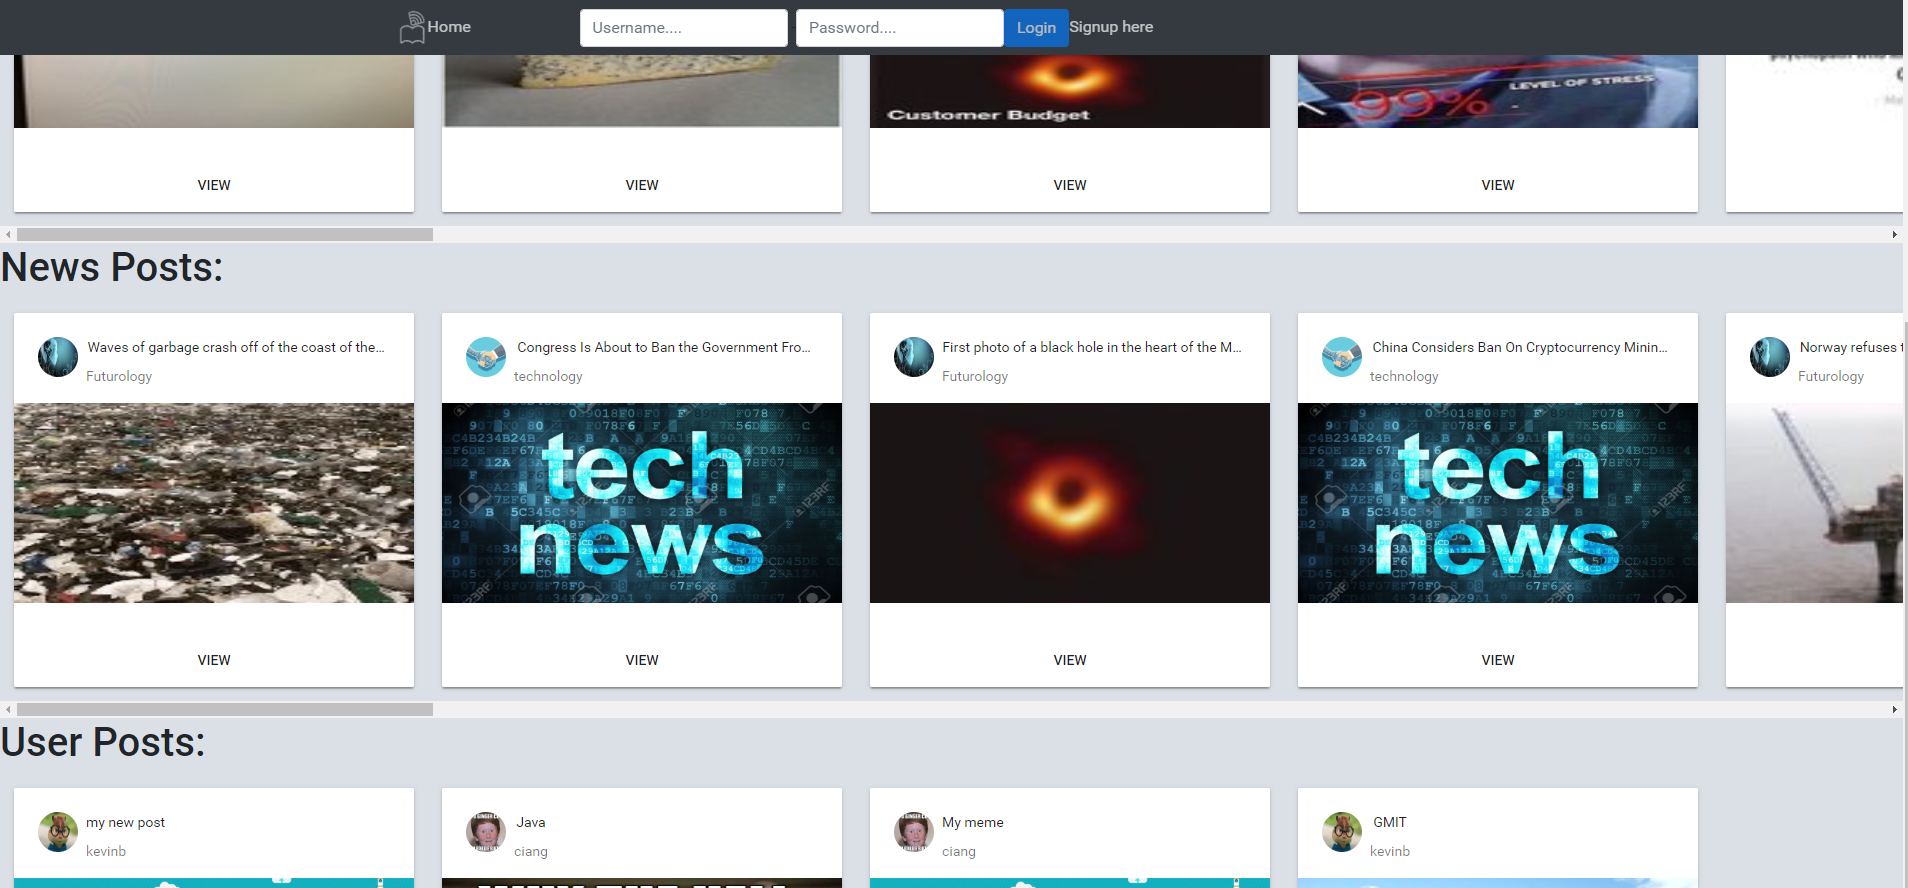
\includegraphics[width=.9\linewidth]{img/ui/headerpcsticky.PNG}
  \captionof{figure}{Sticky Navbar}
  \label{fig:headerStick}
\end{minipage}
\end{figure}

However when the user is logged in even more functionality is active. Shown in Figure  ~\ref{fig:headernodrop} relating general site functions three buttons with corresponding icons are added to redirect the user to the the Home, Make Post and About Us page. For functions related to the current user, a drop down menu was added along with the logged in users thumbnail photo and username. Selecting the arrow icon displayed in Figure\ref{fig:headerdrop} displays a drop down menu. This menu has options to render the Profile, Account Settings, Friends and Saved post pages. The Logout button in the drop down menu logs the user out, deletes the JWT token from session storage and redirects to the homepage. 
\begin{figure}[H]
\centering
\begin{minipage}{.5\textwidth}
  \centering
  
\includegraphics[width=.9\linewidth]{img/ui/headernodrop.PNG}
  \captionof{figure}{Navbar}
  \label{fig:headernodrop}
\end{minipage}%
\begin{minipage}{.5\textwidth}
  \centering
  
\includegraphics[width=.9\linewidth]{img/ui/headerdrop.PNG}
  \captionof{figure}{Navbar Dropdown active}
  \label{fig:headerdrop}
\end{minipage}
\end{figure}



\subsubsection{Log in Page}  \label{loginpage}

The log in page consists of of a username and password input box. In order to submit a login attempt both values must be supplied. The values are then authenticated on the server and if successful the server returns a JWT token that's stored in session storage and the user is redirected to the homepage view.  If the username is invalid the server will return a "Log in failed. User not found." error message to the view or in the case of an invalid password a "Incorrect password" message is returned.
\begin{figure}[H]
\centering
\begin{minipage}{.75\textwidth}
  \centering
  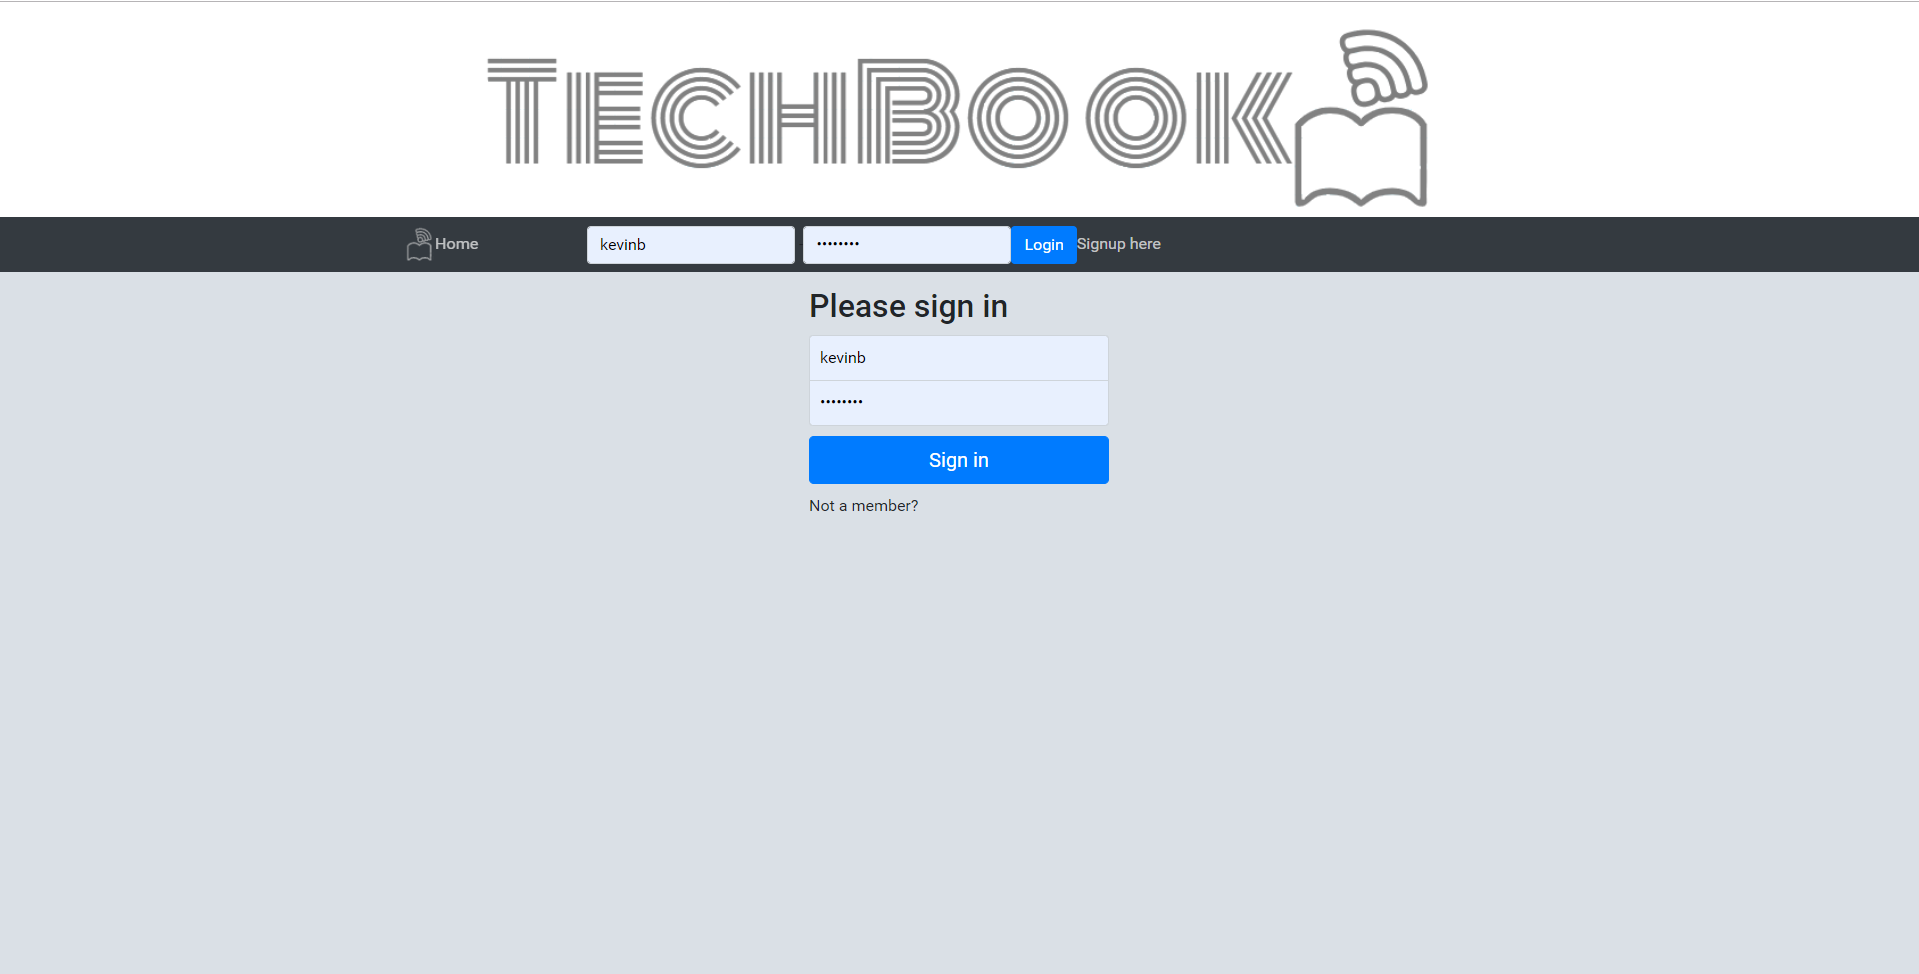
\includegraphics[width=.9\linewidth]{img/ui/login_PC.PNG}
  \captionof{figure}{Web View}
  \label{fig:loginPC}
\end{minipage}%
\begin{minipage}{.25\textwidth}
  \centering
  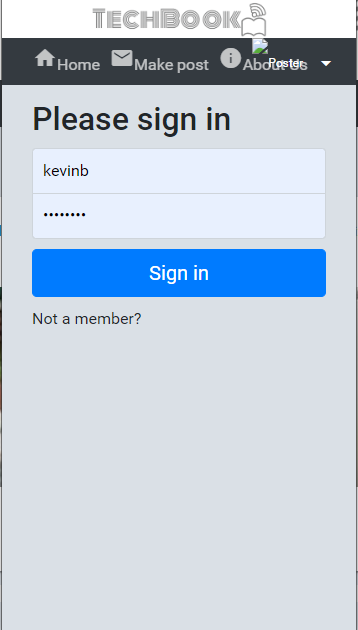
\includegraphics[width=.9\linewidth]{img/ui/login_MOBILE.PNG}
  \captionof{figure}{Mobile view}
  \label{fig:loginMOBILE}
\end{minipage}
\end{figure}

\subsubsection{Register Page}
The register page allows a user to enter credentials for a new user profile. To submit a register attempt all fields are required. This page view contains numerous different aspects that must be validated:


\begin{figure}[H]
\begin{minipage}{.5\textwidth}  %listing bloc will have 50% of the line width 
\lstset{0.6\textwidth, breaklines=true} %set your listing lines widths, and set breaklines to true
\begin{itemize}
\item Username : Required, Must be unique to server.
\item firstname : Required.
\item surname : Required.
\item email : Required, Must contain '@' followed by '.' symbol, Must be unique to server.
\item Password : Must be 8 characters and must match confirm password value.
\end{itemize}

\end{minipage}
\qquad %space between listing bloc and the figure
\begin{minipage}{0.4\textwidth} %figure will have the remaning 40% of the line width
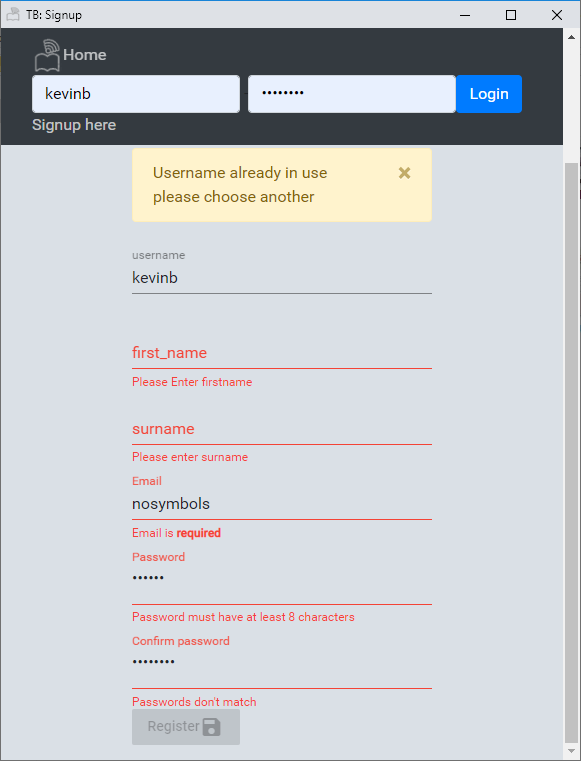
\includegraphics[width=.9\linewidth]{img/ui/signuperror.PNG} %the image must be resized or scaled if needed
\caption{Register Validation}
\end{minipage}
\end{figure}

\begin{figure}[H]
\centering
\begin{minipage}{.75\textwidth}
  \centering
  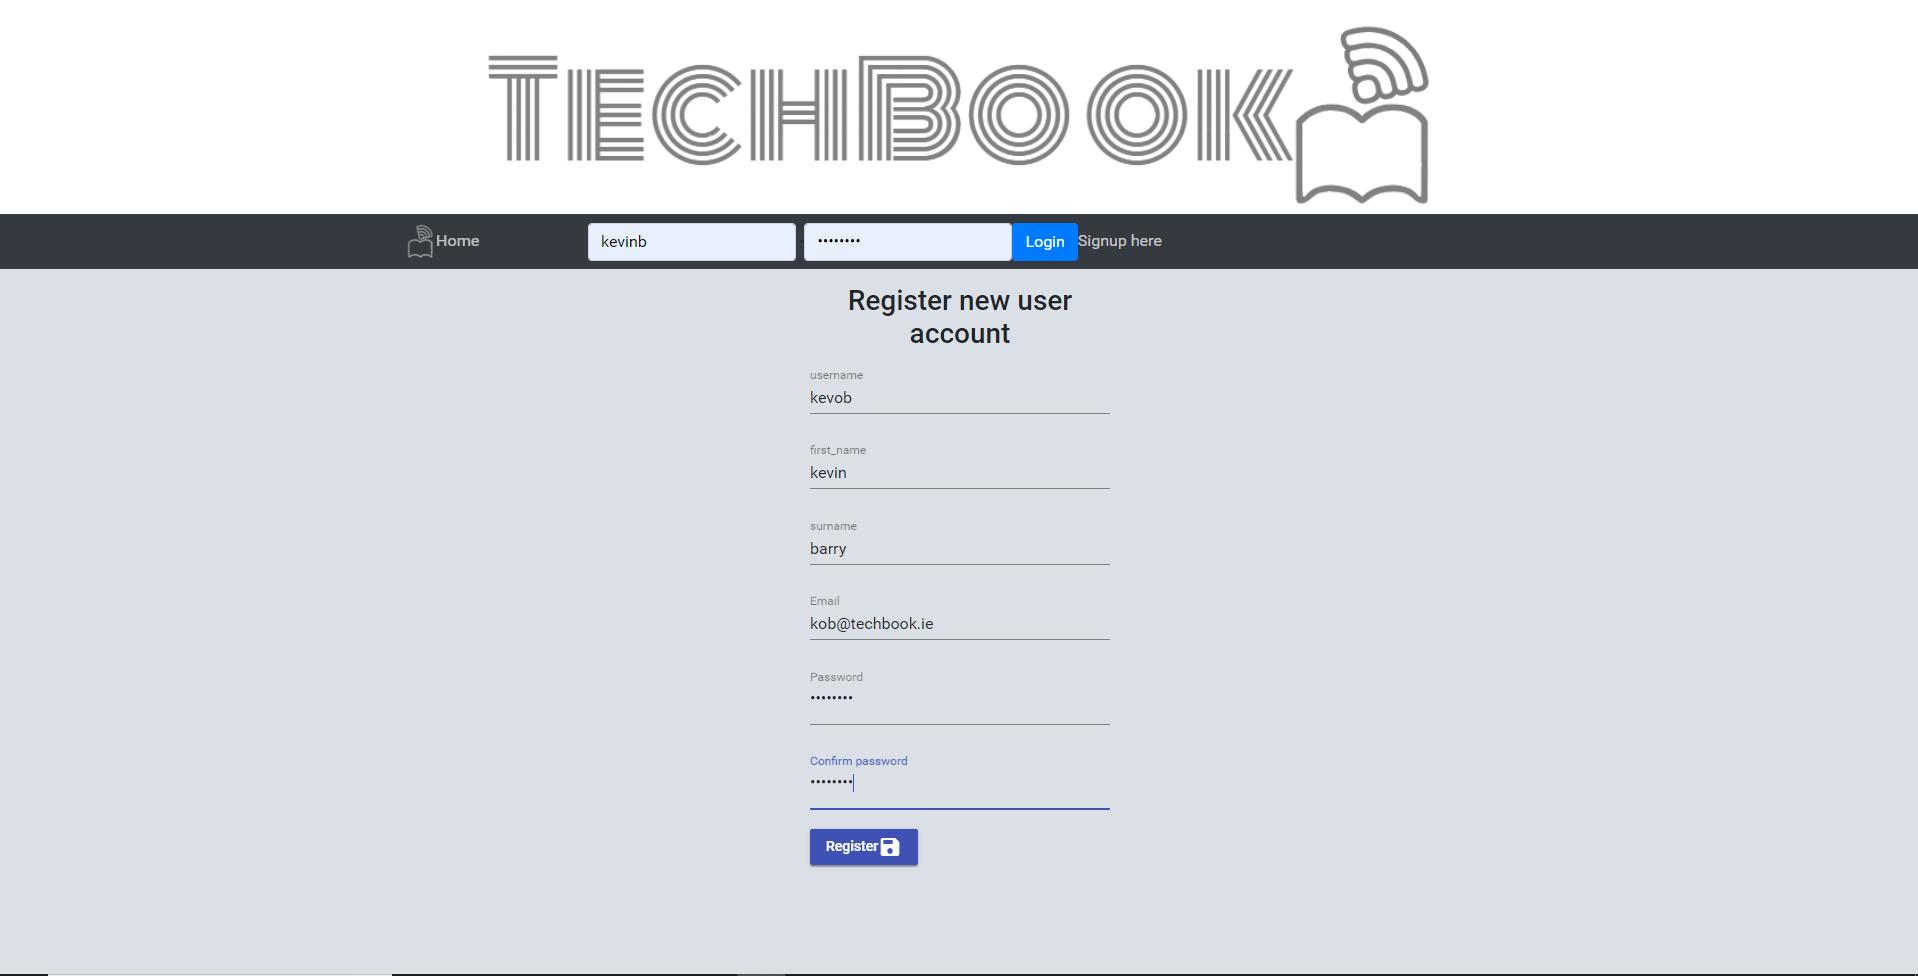
\includegraphics[width=.9\linewidth]{img/ui/sigup_PC.PNG}
  \captionof{figure}{Web View}
  \label{fig:signupPC}
\end{minipage}%
\begin{minipage}{.25\textwidth}
  \centering
  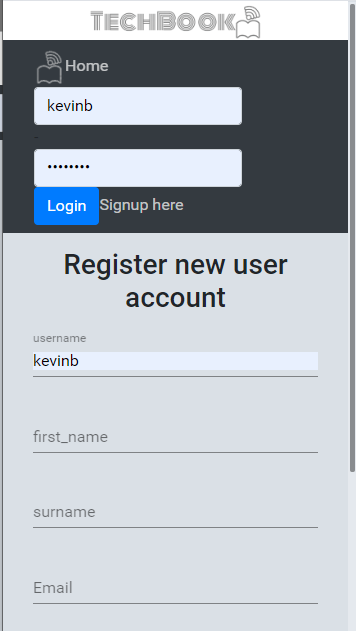
\includegraphics[width=.9\linewidth]{img/ui/signup_MOBILE.PNG}
  \captionof{figure}{Mobile view}
  \label{fig:signupMOBILE}
\end{minipage}
\end{figure}

\subsubsection{Profile Page} 
The profile page is used to view a users details (profile image, avatar, name, username email and when they registered) and activity (created posts and comments on other posts). By using \textbf{Angular Material Components} the page has been split into a grid to display different sections as seen in the Figure \ref{fig:profileHTML} snippet. The grids are assigned to profile info, recent posts and recent comments. Harnessing the functionality of \textbf{Angular Material Components} enables the page to be fully responsive. As you can see in Figure \ref{fig:profilePC} the layout is set to have profile info to the left, while recent comments and posts are stacked on top each other to he right. However as the size of the screen scales, so does the view the grid components that will shrink as the screen size decreases and in the case of a mobile device as seen in Figure \ref{fig:profileMOBILE} the components are stacked vertically on top of one another. 

\begin{lstlisting}[language=HTML,caption={Angular Material Component Grid},captionpos=b,label={fig:profileHTML}]
<div class="mdc-layout-grid">
  <div class="mdc-layout-grid__inner">

    <div class="mdc-layout-grid__cell mdc-layout-grid__cell--span-4">
      <mat-card class="profile-card">
      .......
      </mat-card>
    </div>

    <div class="mdc-layout-grid__cell mdc-layout-grid__cell--span-8">
      <div class="mdc-layout-grid__inner ">
        <div class="mdc-layout-grid__cell mdc-layout-grid__cell--span-12">


          <!-- If the user has made any posts -->
          <div *ngIf="postsUser.length > 0">
            <h1>Recent Posts:</h1>
         ........
          </div>

          <!-- If the user hasn't made any post -->
          <div *ngIf="!postsUser.length > 0">
            <h1>No posts to show</h1>
            <p>Tell {{profile.username}} to get posting!</p>
          </div>
        </div>
        
        <div class="mdc-layout-grid__cell mdc-layout-grid__cell--span-12">

          <!-- If the user has made any comments -->
          <div *ngIf="commentsUser.length > 0">
            <h1>Recent Comments:</h1>
            <!-- Comment card -->
            <mat-card class="comment-card" *ngFor="let commentUser of commentsUser">
              ......
            </mat-card>
          </div>

          <!-- If the user hasn't made any comments -->
            <h1>No comments to show</h1>

          </div>
        </div>
      </div>
    </div>
  </div><div *ngIf="!commentsUser.length > 0">
          
</div>
\end{lstlisting}

The profile page is used for both viewing a users own profile and viewing another users profile and is changed dynamically. When viewing another users account a follow/unfollow option appears. Once a user follows another user the button changes to unfollow and visa versa. Viewing your own profile disables these options and allows the user to view pages they are subscribed to. This is achieved by a method in the \textit{userService} shown in Figure \ref{fig:profileJWT} that checks if there is a valid JWT or \textit{Json Web Token} for that user and adjust the options accordingly Figure \ref{fig:profilefollow}.

\begin{lstlisting}[language=JAVASCRIPT,caption={Validate JWT},captionpos=b,label={fig:profileJWT}]
  // Check if a user is logged in
  isLoggedIn(): boolean {
    var currentToken = this.getJwtToken();
    if (currentToken) {
      return true;
    } else {
      return false;
    }
  }
  \end{lstlisting}
\begin{lstlisting}[language=HTML,caption={Follow / Unfollow option},captionpos=b,label={fig:profilefollow}]
       <mat-card-actions>
          <!-- If user is logged in -->
          <div *ngIf="userAPI.isLoggedIn()">
            <button mat-button [routerLink]="['/saved/', profile.username]">SUBSCRIBED POSTS</button>
            <button mat-button [routerLink]="['/follow/', profile.username]">FRIENDS</button>
            <button *ngIf="!isFollowing && !isUser" mat-button (click)="follow(profile._id)">FOLLOW</button>
            <button *ngIf="isFollowing && !isUser" mat-button (click)="unFollow(profile._id)">UNFOLLOW</button>
          </div>
          <!-- If user is not logged in -->
          <div class="user-buttons" *ngIf="!userAPI.isLoggedIn()">
            <button mat-button [routerLink]="['/saved/', profile.username]">SUBSCRIBED POSTS</button>
            <button mat-button [routerLink]="['/follow/', profile.username]">FOLLOW STUFF</button>
          </div>
        </mat-card-actions>
\end{lstlisting}

\begin{figure}[H]
\centering
\begin{minipage}{.75\textwidth}
  \centering
  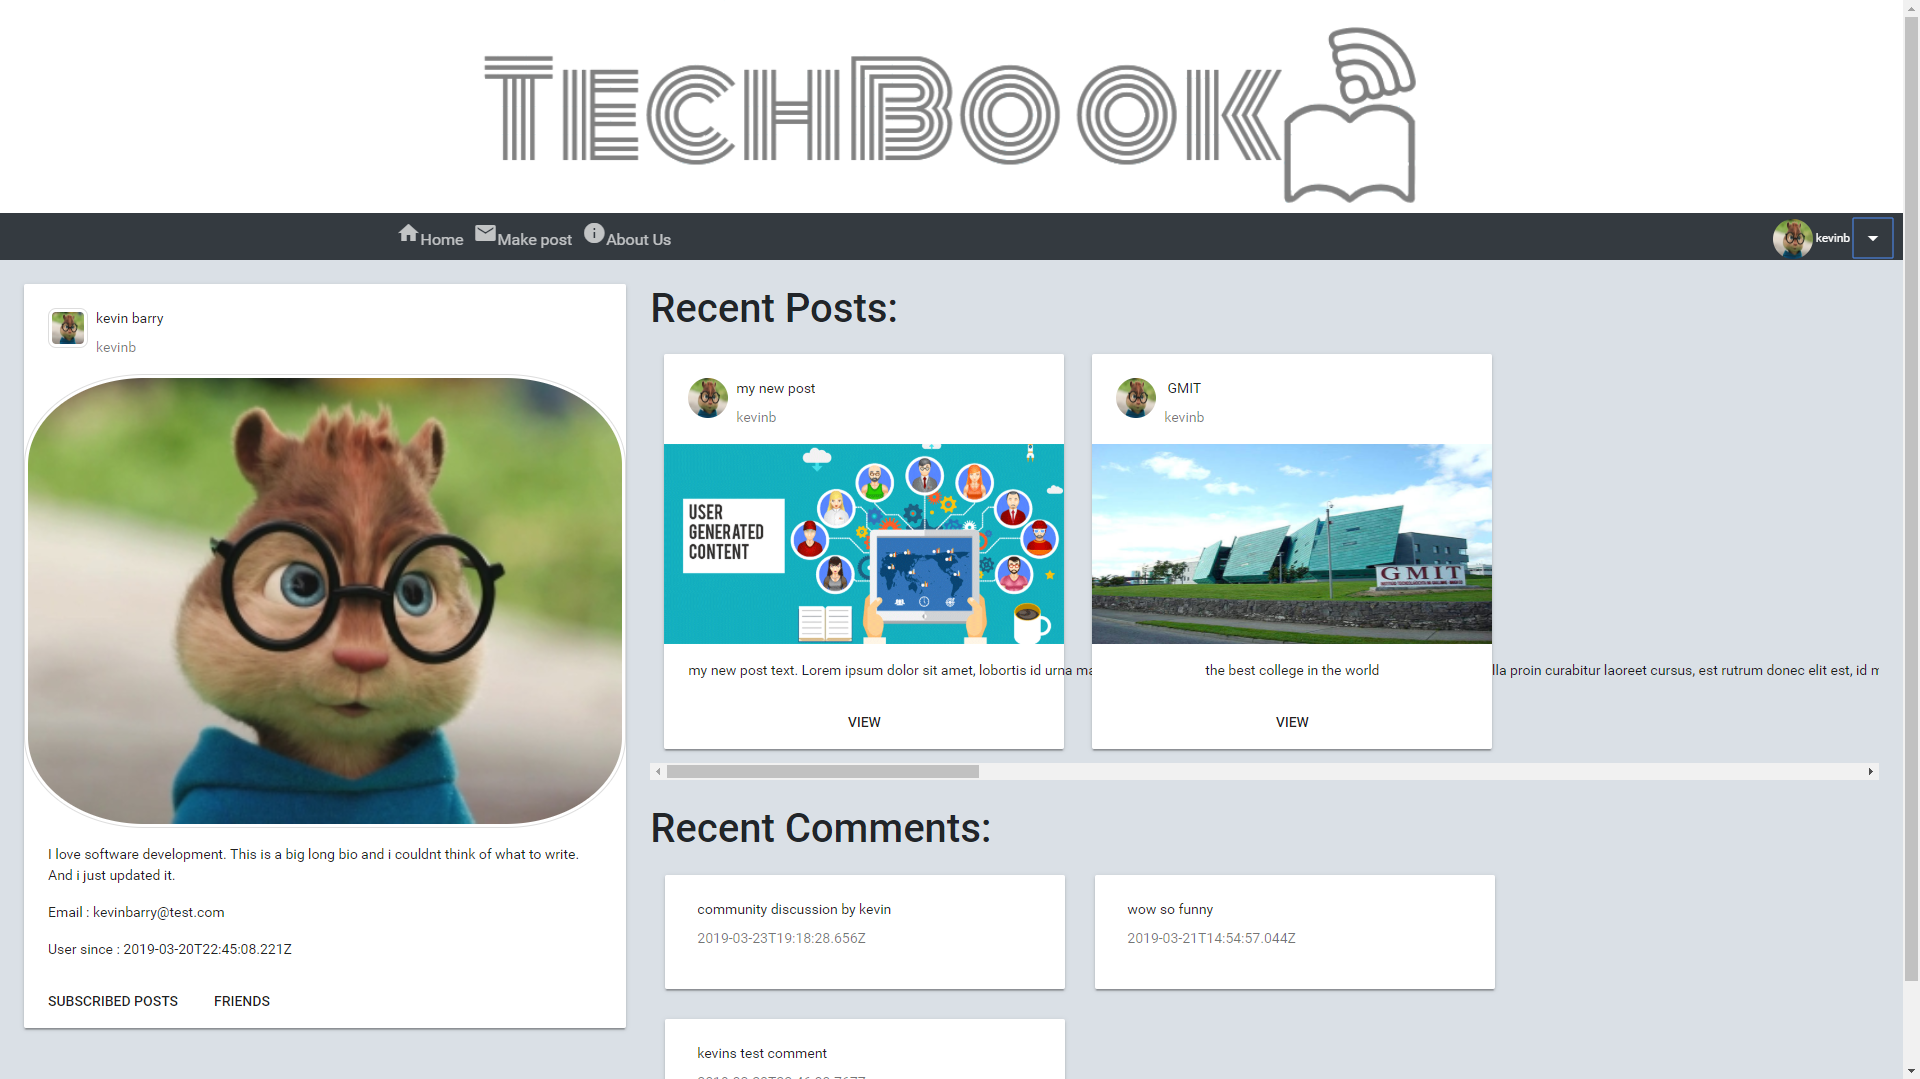
\includegraphics[width=.9\linewidth]{img/ui/profile_PC.PNG}
  \captionof{figure}{Web View}
  \label{fig:profilePC}
\end{minipage}%
\begin{minipage}{.25\textwidth}
  \centering
  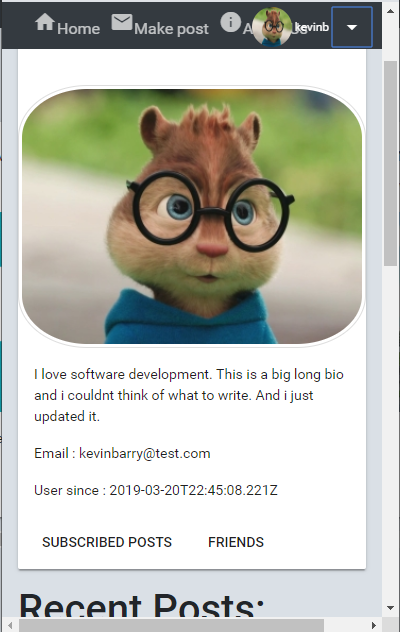
\includegraphics[width=.9\linewidth]{img/ui/profile_MOBILE.PNG}
  \captionof{figure}{Mobile view}
  \label{fig:profileMOBILE}
\end{minipage}
\end{figure}

\subsubsection{Settings Page}
The settings page view allows a user to edit their current credentials and is accessed by clicking the settings tab on the navbar drop down menu. The form fields are pre-filled from the users data retrieved by the server.

\begin{lstlisting}[language=JavaScript,caption={Auto fill form data},captionpos=b,label={fig:userscema}]
/**
 * Set the form data in SettingsForm to the details of the current user.
 * 
 * @param id The current users id.
 */
setForm(id) {
  this.userService.getProfile(id)
    .subscribe(profile => {
      // Must extract profile data from response.
      this.profileinfo = profile[0];
      // Form object
      this.settingsForm.setValue({
        email: this.profileinfo.email,
        first_name: this.profileinfo.first_name,
        surname: this.profileinfo.surname,
        bio: this.profileinfo.bio
      });
    });
}
\end{lstlisting}
 This page also allows the user to update or change their current profile image. Selecting the 'choose file' button pops up a file explorer window and allows the user to select an image. The chosen image is then shown in a preview tab so the user can have a peek prior to selecting the "Upload new profile image" button. This was achieved by importing the \textbf{ng2-file-upload} module and applying custom functions. The uploaded image is then saved in a image folder on the server and the users account is updated with the location to access this image. The uploader is also validated to only accept image files.
\begin{figure}[H]
\centering
\begin{minipage}{.75\textwidth}
  \centering
  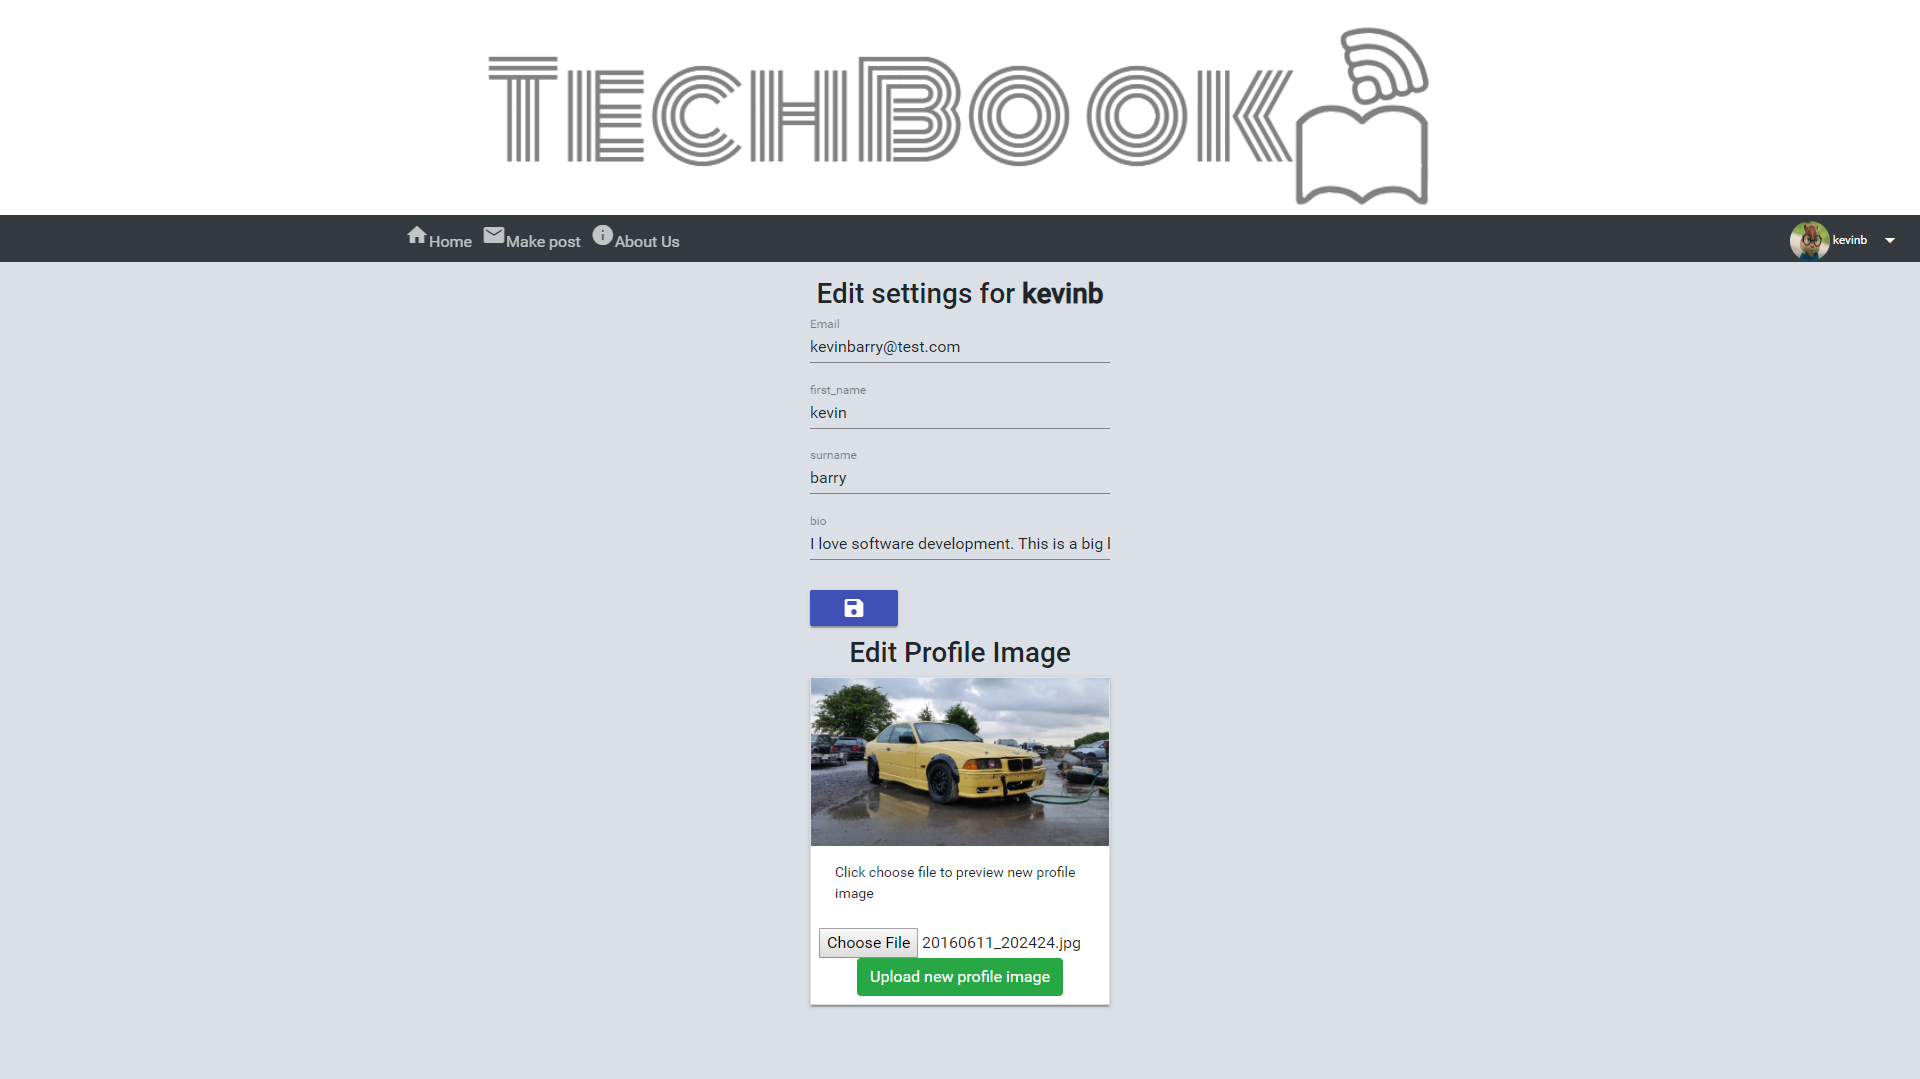
\includegraphics[width=.9\linewidth]{img/ui/settings_PC.PNG}
  \captionof{figure}{Web View}
  \label{fig:settingsPC}
\end{minipage}%
\begin{minipage}{.25\textwidth}
  \centering
  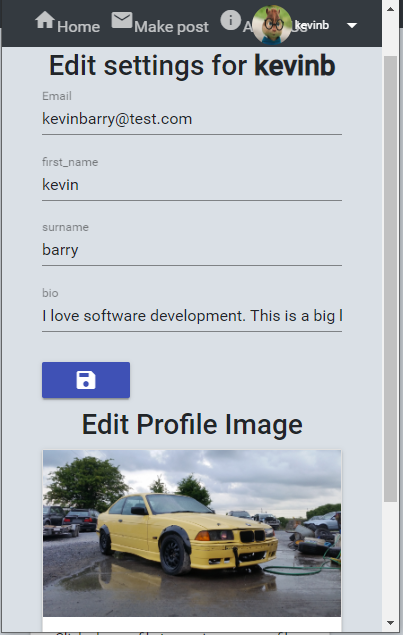
\includegraphics[width=.9\linewidth]{img/ui/settings_MOBILE.PNG}
  \captionof{figure}{Mobile view}
  \label{fig:settingsMOBILE}
\end{minipage}
\end{figure}

\subsubsection{Friends Page} 
The friends page is a view that allows a user to toggle a view between followers and following. This page can be accessed in two ways which render different views. If a user wants to view a list of their own followers and who they are following they can select the "Friends" button in the navbar drop down menu. If a user would like to view another users followers and following list a button "Follows" can be selected on the preferred users profile page. The lists contain cards that show a image avatar, username and bio for each user. To view a users profile from this view simply click on the username and the system redirects you to that users profile page.
\begin{figure}[H]
\centering
\begin{minipage}{.75\textwidth}
  \centering
  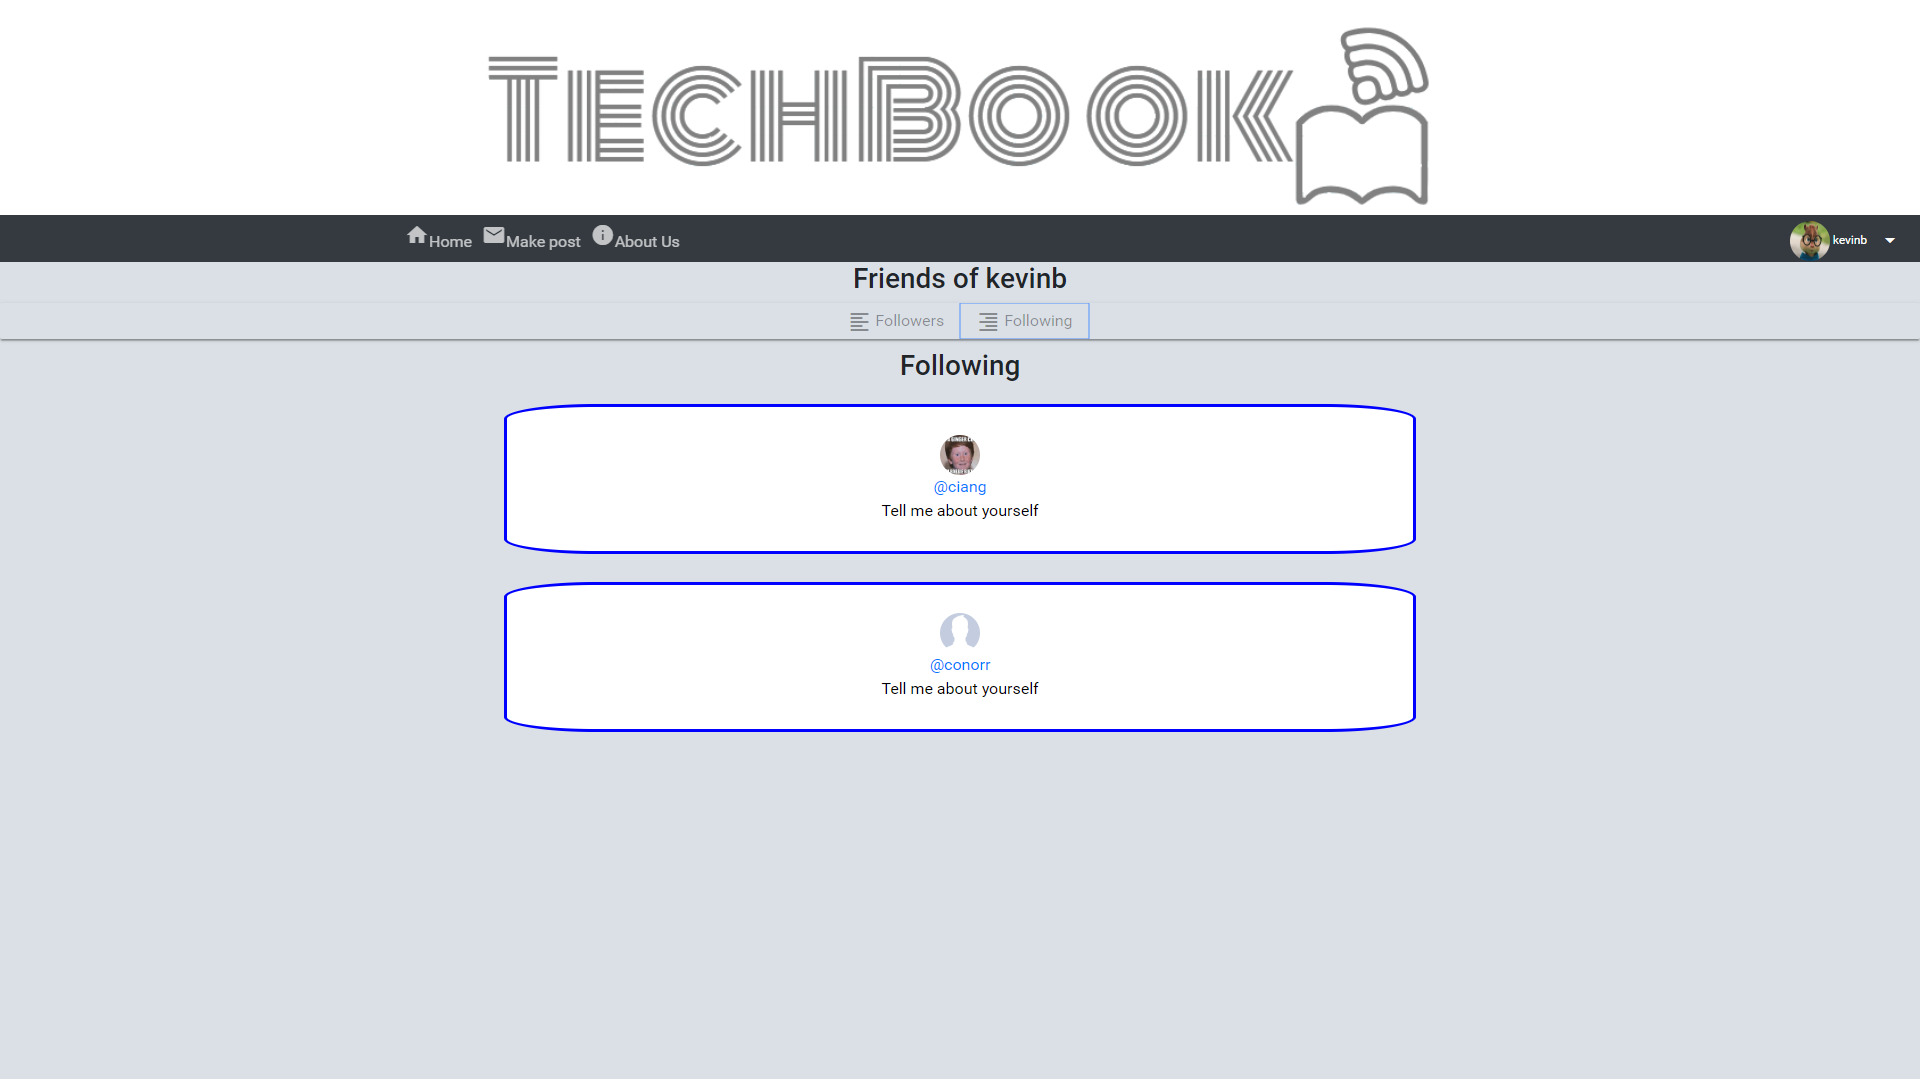
\includegraphics[width=.9\linewidth]{img/ui/followPC.PNG}
  \captionof{figure}{Web View}
  \label{fig:followPC}
\end{minipage}%
\begin{minipage}{.25\textwidth}
  \centering
  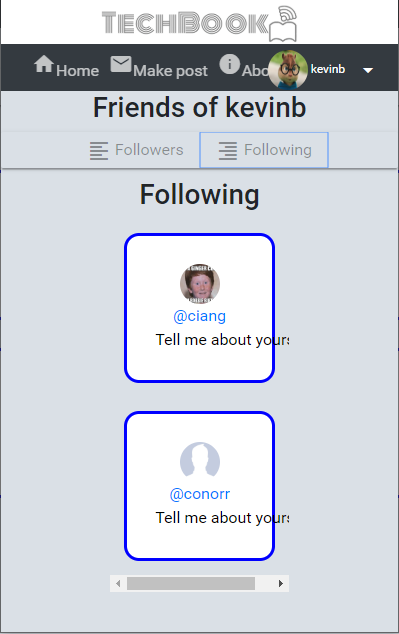
\includegraphics[width=.9\linewidth]{img/ui/followMOBILE.PNG}
  \captionof{figure}{Mobile view}
  \label{fig:followMOBILE}
\end{minipage}
\end{figure}

\subsubsection{Home Page}

\begin{figure}[H]
\centering
\begin{minipage}{.75\textwidth}
  \centering
  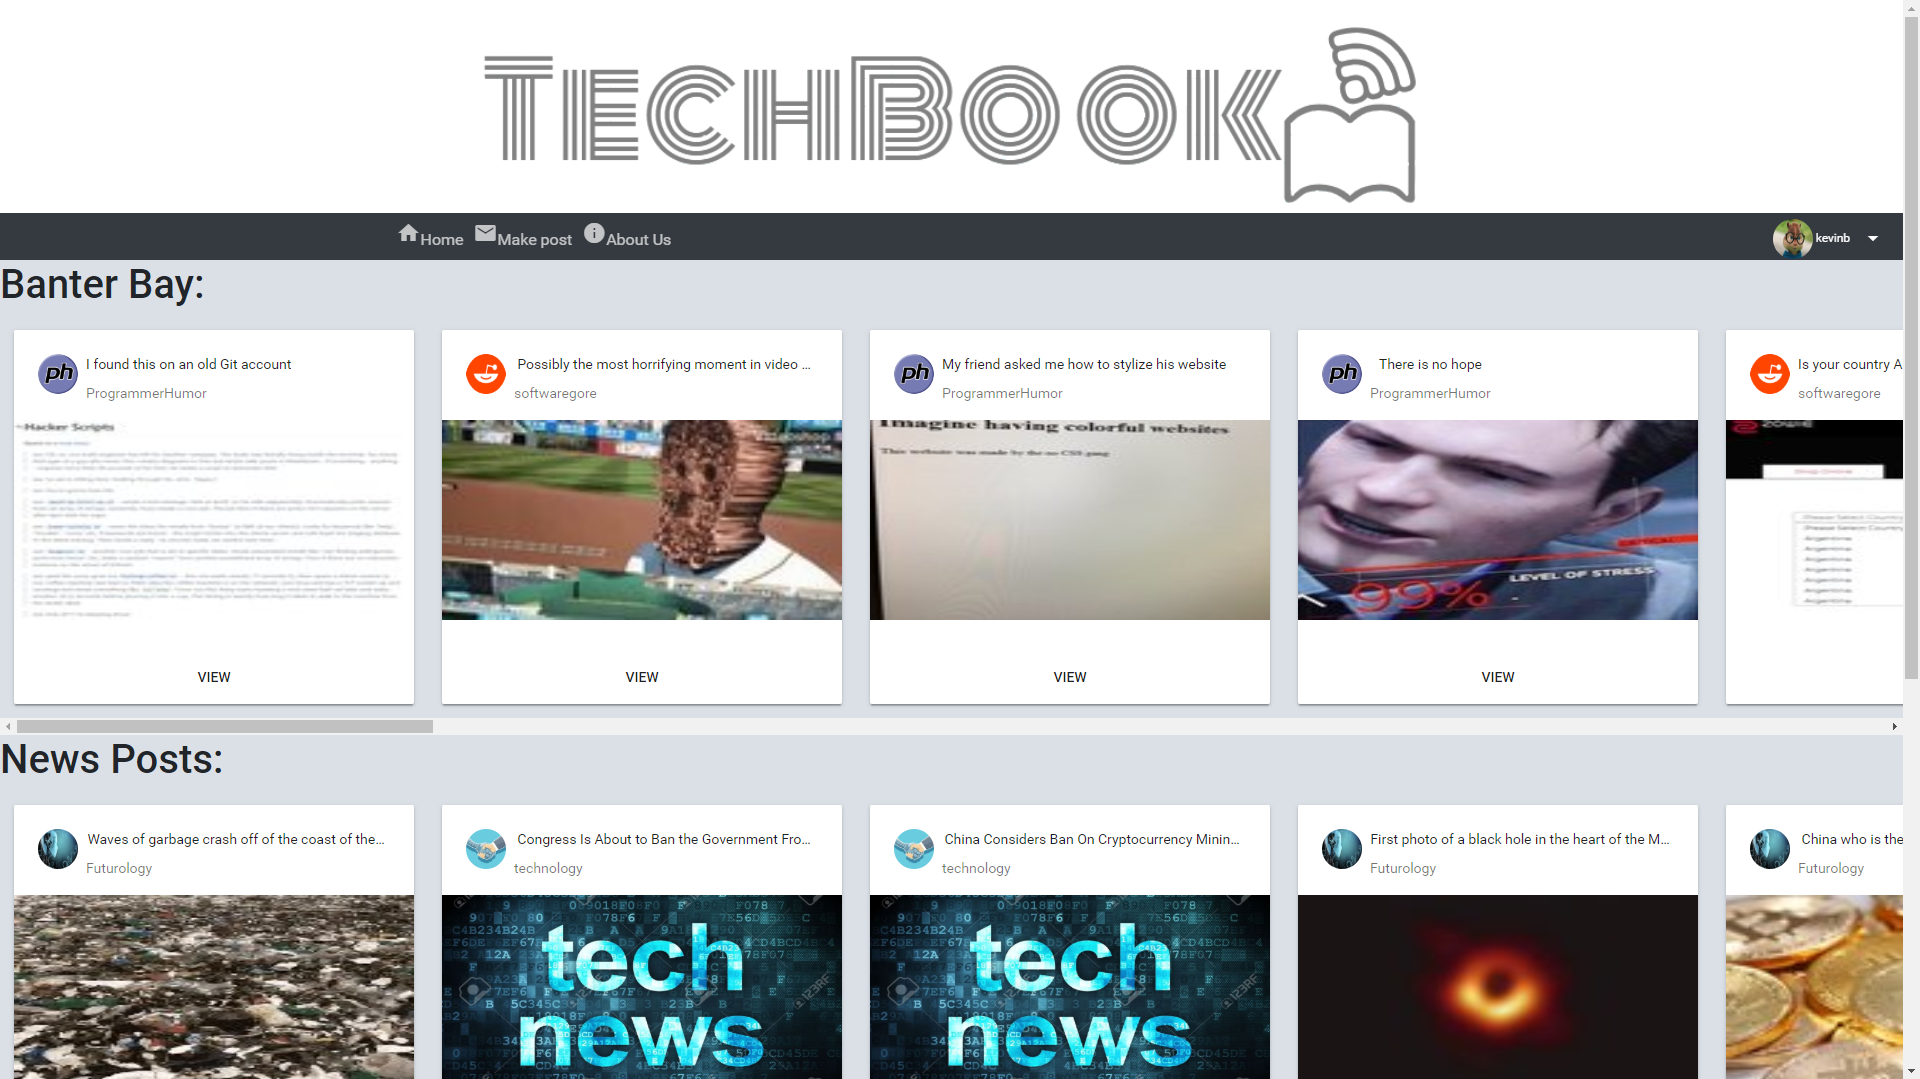
\includegraphics[width=.9\linewidth]{img/ui/homepcsnap.PNG}
  \captionof{figure}{Web View}
  \label{fig:test1}
\end{minipage}%
\begin{minipage}{.25\textwidth}
  \centering
  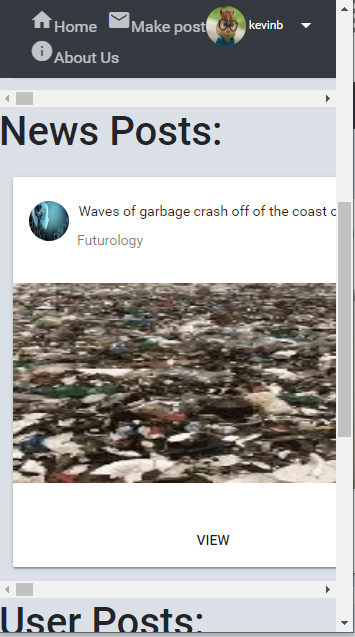
\includegraphics[width=.9\linewidth]{img/ui/homemobile.PNG}
  \captionof{figure}{Mobile view}
  \label{fig:test2}
\end{minipage}
\end{figure}

\subsubsection{Posts Page}
\subsubsection{About Page}
The purpose of the about page view is to give the user an insight into the project. The view is separated into three sections with each item being displayed on its own card. Each card consists of an image, a link to the resource, a summary of the resource link and also some brief information on that item. The Team section is a over view of the developers of the web application with clickable link to view our Github profiles. The Documentation section contains links to the project source code, dissertation and the Swagger documentation for the API. The third section is used to provide links to resources and give information on some of the components used in the project such as  MEAN Stack, MongoDB, Express.js, Angular, Node.JS, Reddit API, Passport.JS, HTML and CSS.
\begin{figure}[H]
\centering
\begin{minipage}{.75\textwidth}
  \centering
  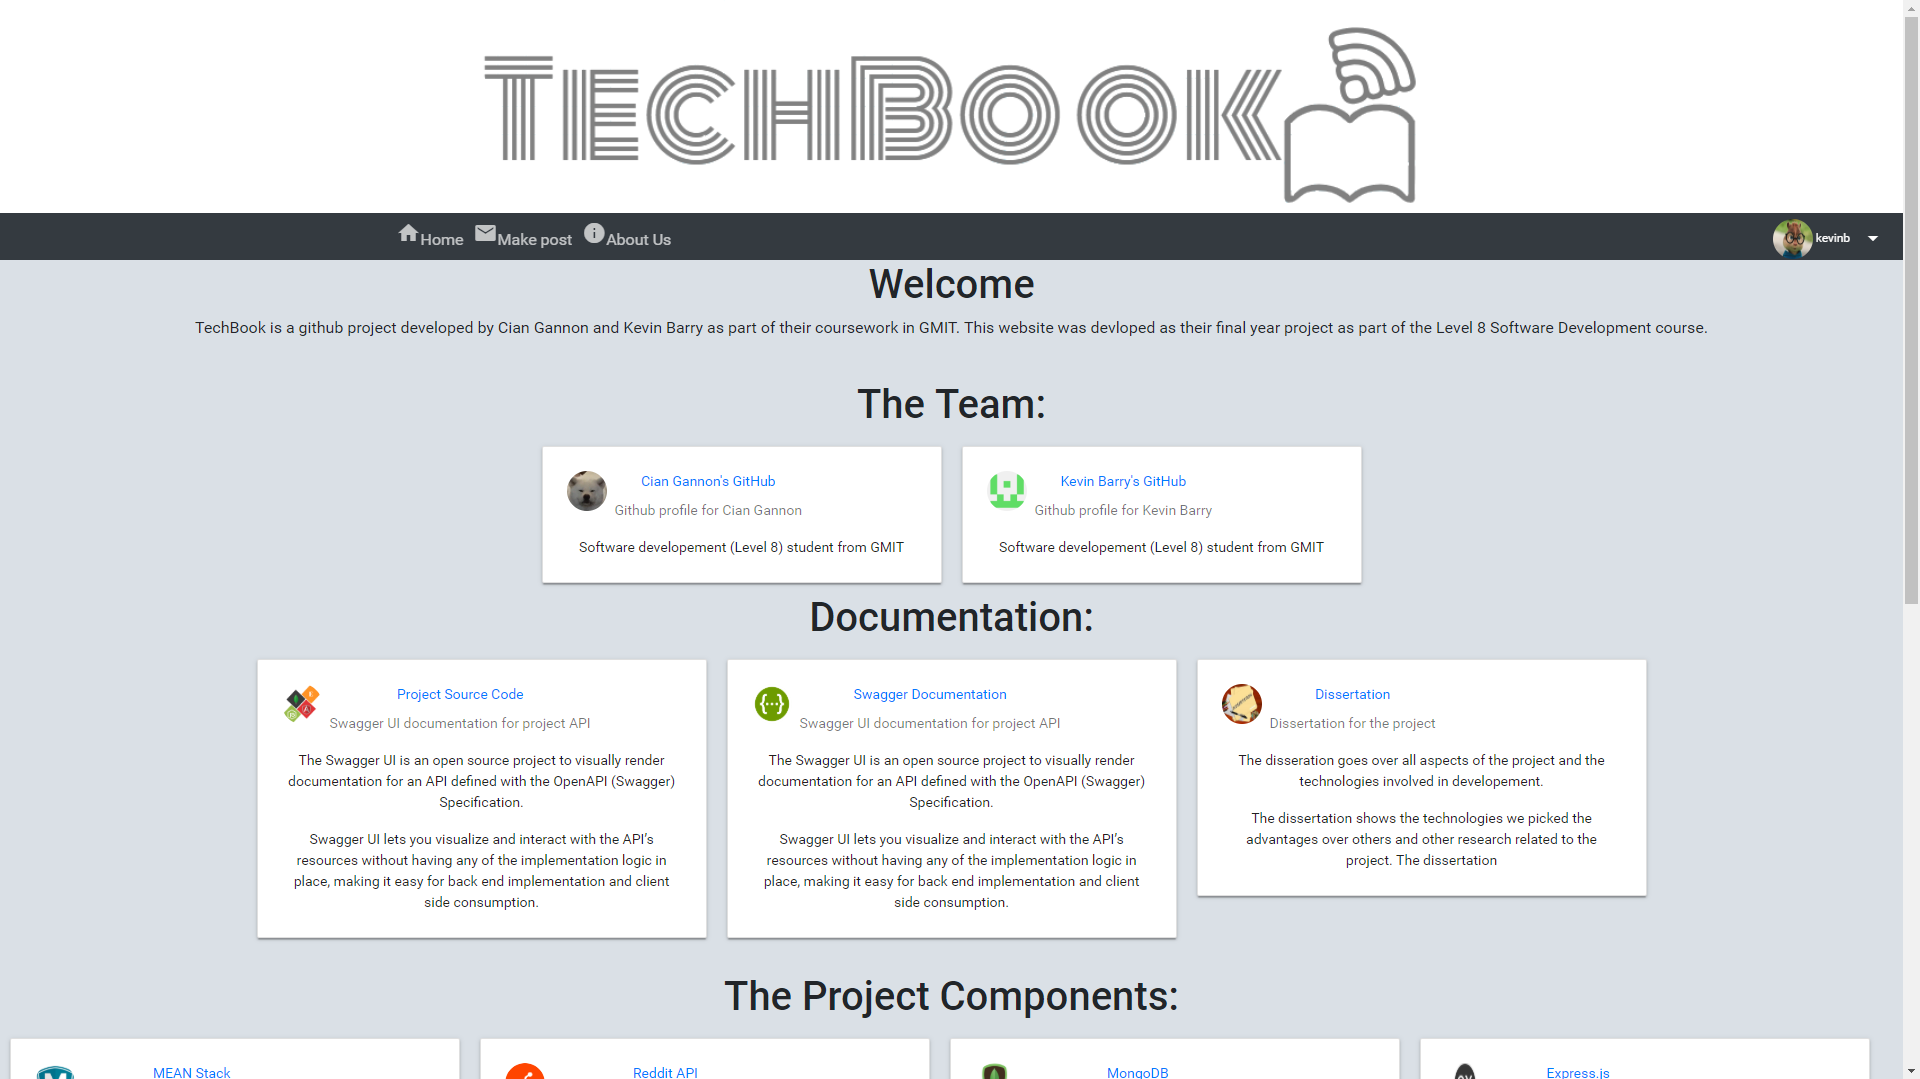
\includegraphics[width=.9\linewidth]{img/ui/about_PC.PNG}
  \captionof{figure}{Web View}
  \label{fig:aboutPC}
\end{minipage}%
\begin{minipage}{.25\textwidth}
  \centering
  
\includegraphics[width=.9\linewidth]{img/ui/about_MOBILE.PNG}
  \captionof{figure}{Mobile view}
  \label{fig:aboutMobile}
\end{minipage}
\end{figure}
\begin{itemize}
\item Architecture, UML etc. An overview of the different components of the system. Diagrams etc… Screen shots etc.
\end{itemize}

\begin{table}[h]
  \centering
  \begin{tabular}{x{2cm}p{3cm}}
    \toprule \\
    Column 1 & Column 2 \\
    \midrule \\
    Rows 2.1 & Row 2.2 \\
    \bottomrule
  \end{tabular}
  \caption{A table.}
  \label{table:mytable}
\end{table}